\documentclass[tikz,border=2pt]{standalone}
\usepackage{amsmath}
\usepackage{pgfplots}
\pgfplotsset{compat=1.18}

\begin{document}
% f(x) = x^2: near x_0 = 1 (f' != 0) nearby equations f(x) = b have exactly one nearby solution
% (locally bijective); near the fold x_0 = 0 (f' = 0) values b > 0 have two nearby solutions
% and b < 0 none, so f is neither locally injective nor locally surjective there.
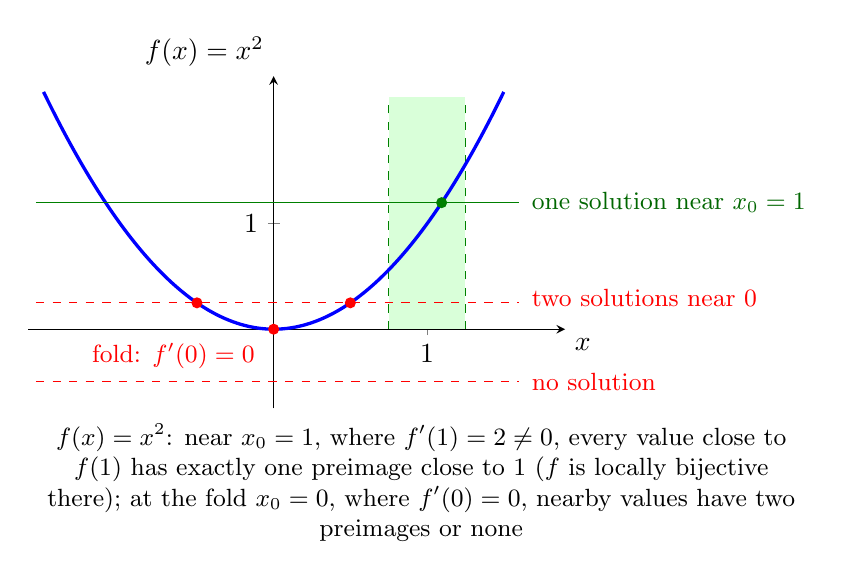
\begin{tikzpicture}
	\begin{axis}[
		axis lines=middle, xmin=-1.6, xmax=1.9, ymin=-0.75, ymax=2.4,
		xtick={1}, ytick={1},
		xlabel={$x$}, ylabel={$f(x)=x^2$}, xlabel style={below right}, ylabel style={above left},
		samples=120, smooth, width=8.4cm, height=5.8cm, clip=false
		]
		\fill[green!15] (axis cs:0.75,0) rectangle (axis cs:1.25,2.2);
		\draw[green!50!black, dashed] (axis cs:0.75,0) -- (axis cs:0.75,2.2);
		\draw[green!50!black, dashed] (axis cs:1.25,0) -- (axis cs:1.25,2.2);
		\addplot[blue, very thick, domain=-1.5:1.5] {x^2};
		\draw[green!50!black] (axis cs:-1.55,1.2) -- (axis cs:1.6,1.2);
		\fill[green!50!black] (axis cs:1.095,1.2) circle (2pt);
		\node[green!40!black, font=\small, anchor=west] at (axis cs:1.62,1.2) {one solution near $x_0=1$};
		\draw[red, dashed] (axis cs:-1.55,0.25) -- (axis cs:1.6,0.25);
		\fill[red] (axis cs:0.5,0.25) circle (2pt);
		\fill[red] (axis cs:-0.5,0.25) circle (2pt);
		\node[red, font=\small, anchor=west] at (axis cs:1.62,0.3) {two solutions near $0$};
		\draw[red, dashed] (axis cs:-1.55,-0.5) -- (axis cs:1.6,-0.5);
		\node[red, font=\small, anchor=west] at (axis cs:1.62,-0.5) {no solution};
		\fill[red] (axis cs:0,0) circle (2pt);
		\node[red, font=\small, anchor=north east] at (axis cs:-0.06,-0.04) {fold: $f'(0)=0$};
	\end{axis}
	\node[anchor=north, font=\small, align=flush center, text width=9.6cm] at ([yshift=-2pt]current axis.outer south) {$f(x)=x^2$: near $x_0=1$, where $f'(1)=2\neq0$, every value close to $f(1)$ has exactly one preimage close to $1$ ($f$ is locally bijective there); at the fold $x_0=0$, where $f'(0)=0$, nearby values have two preimages or none};
\end{tikzpicture}
\end{document}
